%!TEX root = ../Pflichtenheft.tex

\chapter{Produktübersicht}

Die Kernfunktionalität des \NewsGenie ist die Beantwortung von in natürlicher
Sprache gestellten Benutzeranfragen zur aktuellen Nachrichtenlage. Wie im
Use-Case-Diagramm \textit{User stellt Frage an \NewsGenie}, Abb. \ref{uc-frage}, 
dargestellt, meldet sich der Benutzer dafür an einem Client an und kann dann
Fragen in natürlicher Sprache stellen. Diese werden vom Client in Text
umgewandelt und an den Server geschickt. Der Server verarbeitet die Anfrage, 
stellt Nachfragen oder liest, falls die gesuchte Information ausreichend
eingegrenzt ist, einen Artikel vor.
Die Abfolge einer solchen Anfrage wird im Aktivitätsdiagramm \textit{User stellt
Frage an \NewsGenie}, Abb \ref{akt-frage},  genauer dargestellt.

\begin{figure}[h]
\centering
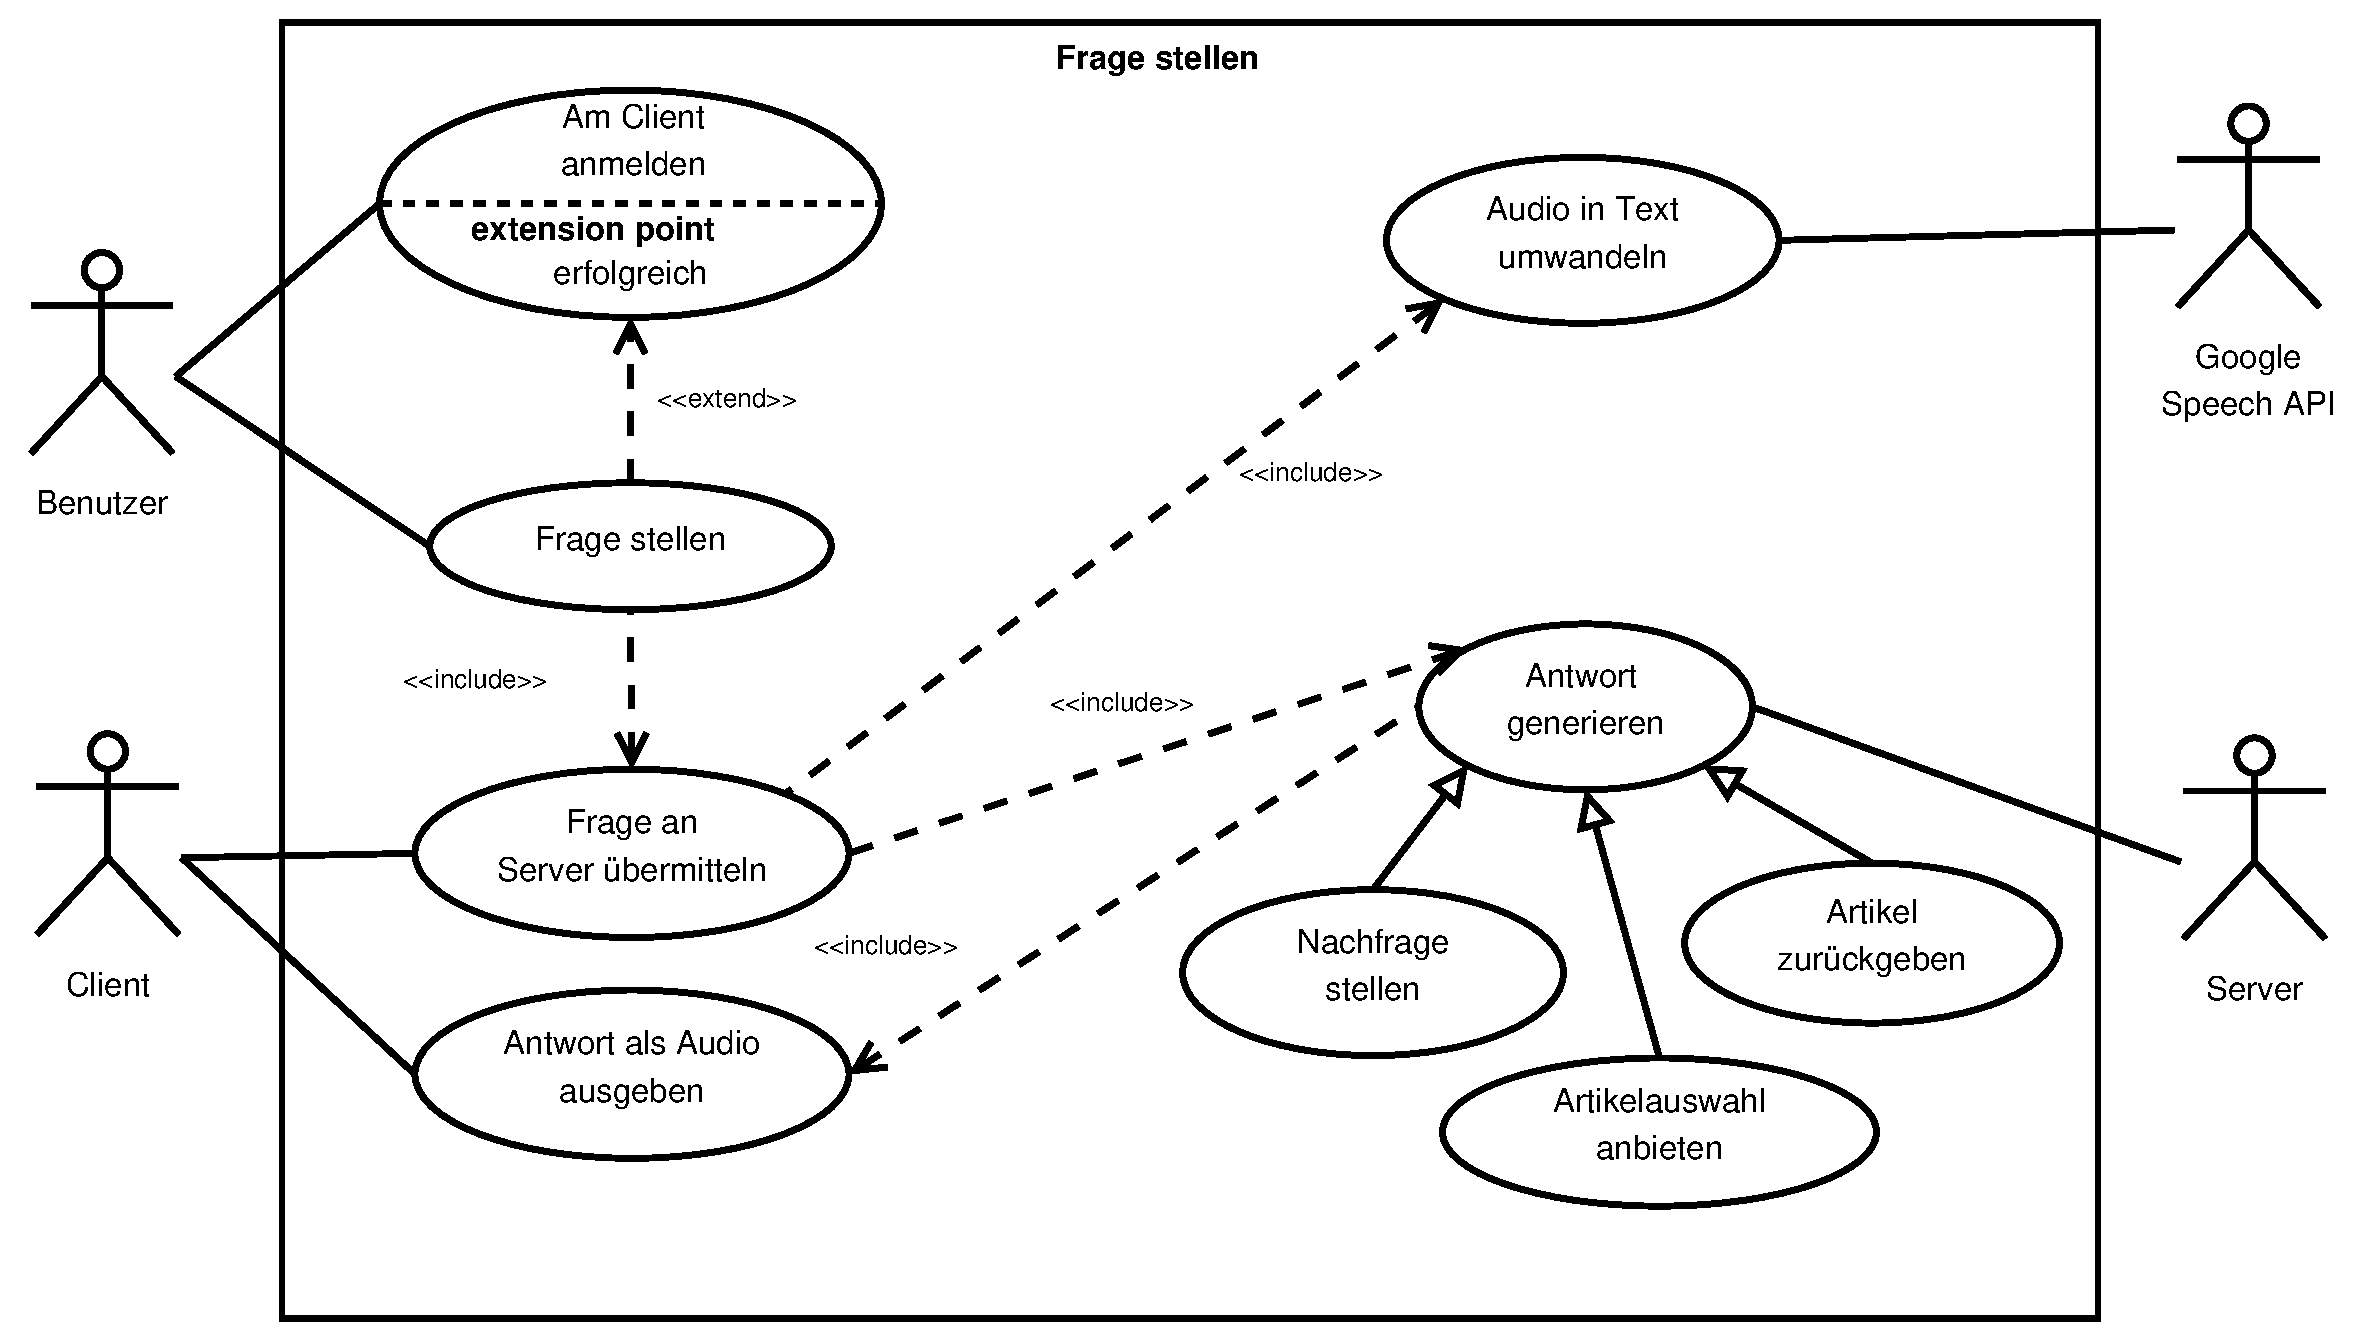
\includegraphics[width=1\textwidth]{Pflichtenheft/03_produktuebersicht/frage_stellen}
\caption{Use-Case, \textit{User stellt Frage an \NewsGenie} \label{uc-frage}}
\end{figure}


\begin{figure}[h]
\centering
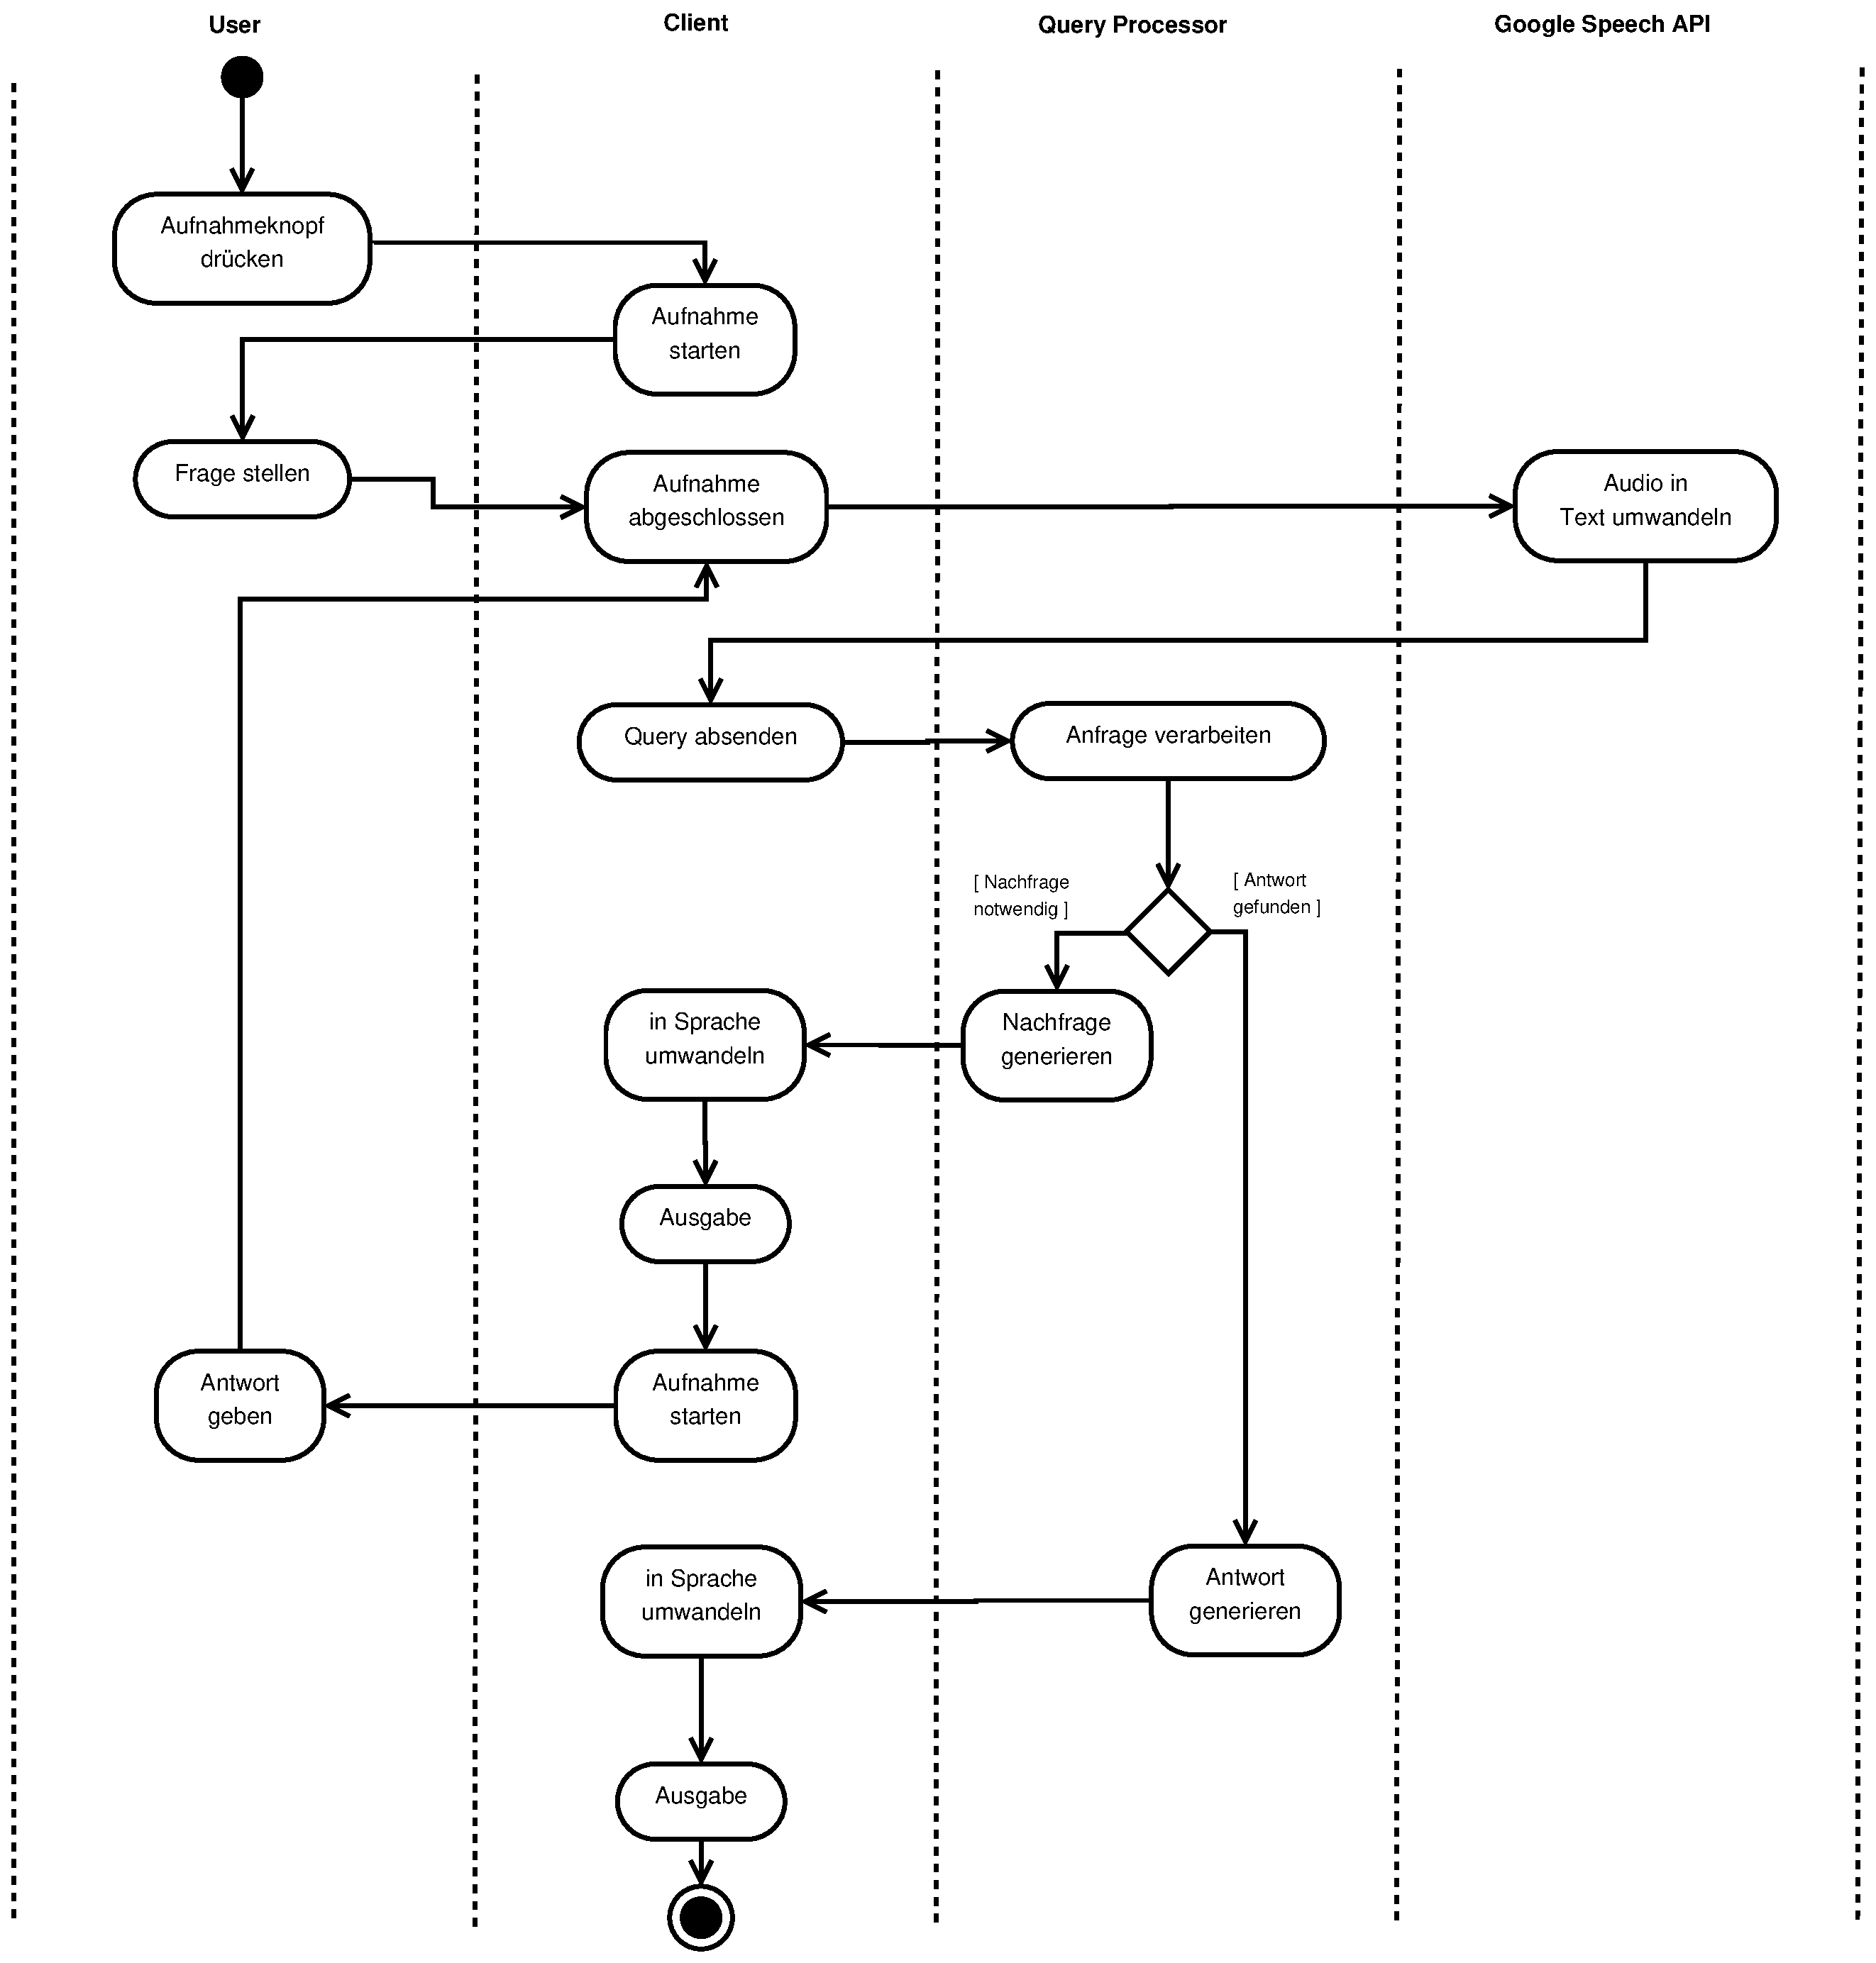
\includegraphics[width=1\textwidth]{Pflichtenheft/03_produktuebersicht/ablauf_frage}
\caption{Aktivitätsdiagramm, \textit{User stellt Frage an \NewsGenie}
\label{akt-frage}}
\end{figure}

\FloatBarrier

Neben der Verarbeitung der Anfragen verfügt der Server über ein Crawler-Backend,
welches die von den Benutzern hinzugefügten RSS-Feeds und darin verlinkte
Artikel in regelmäßigen Abständen besucht, archiviert und indexiert. Im Use-Case
\textit{Backend}, Abb \ref{uc-backend} wird dies dargestellt.

\begin{figure}[h]
\centering
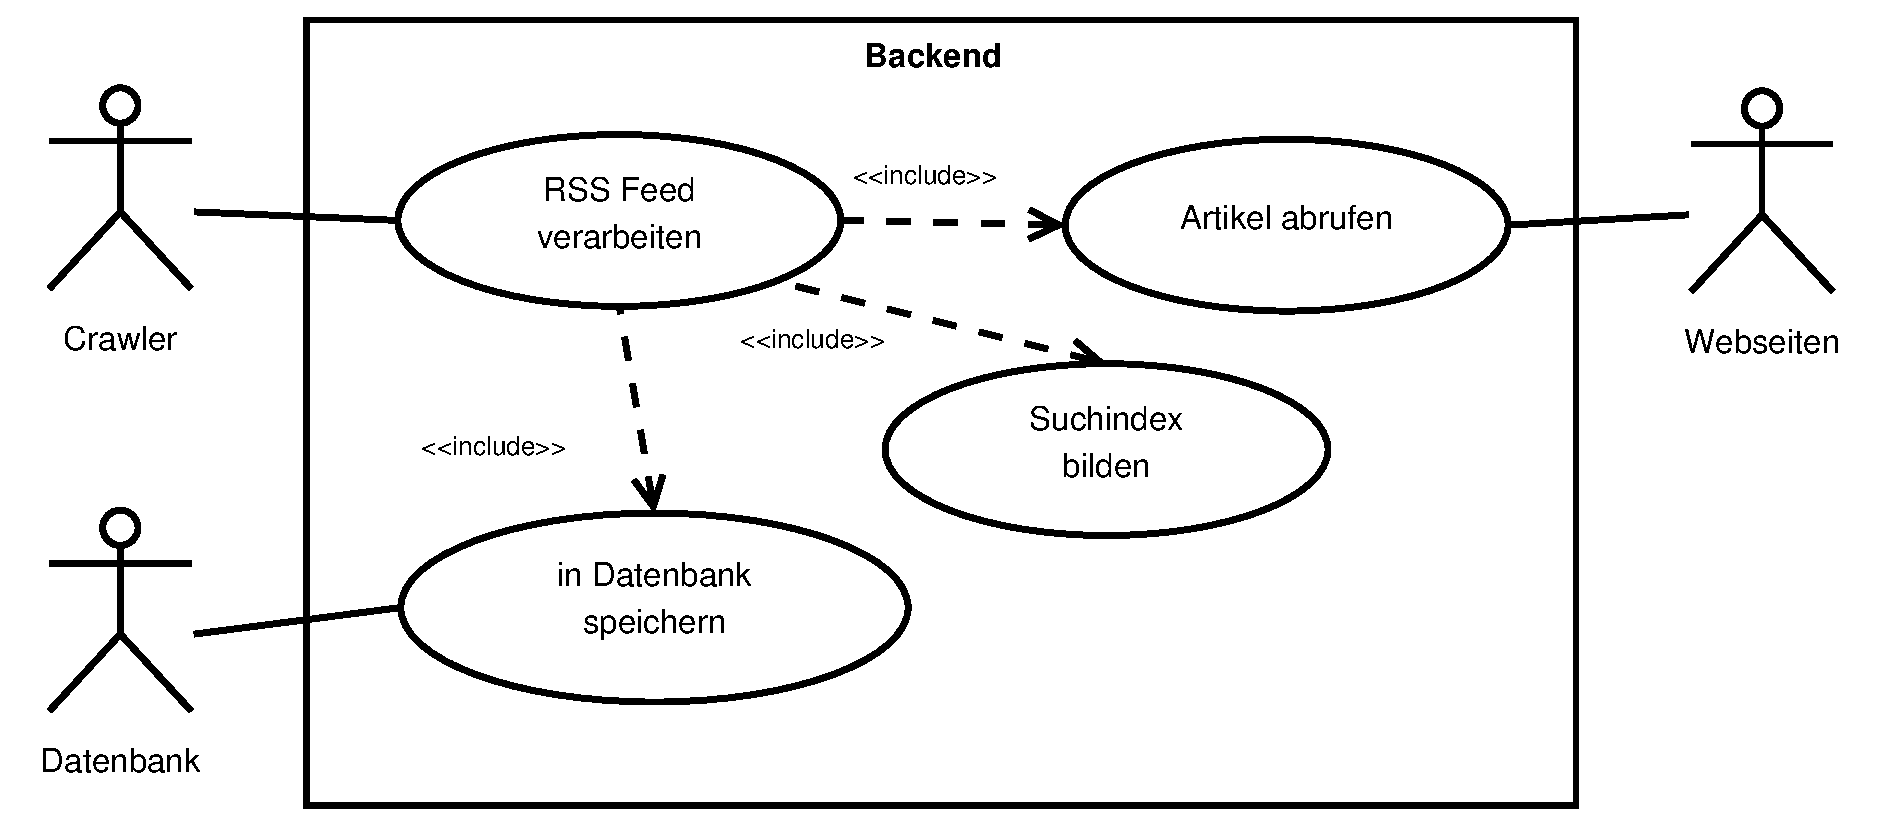
\includegraphics[width=1\textwidth]{Pflichtenheft/03_produktuebersicht/backend}
\caption{Use-Case, \textit{Backend} \label{uc-backend}}
\end{figure}

\FloatBarrier

Da die Konfiguration der Anwendung durch reine Spracheingaben sehr mühsam wäre,
bietet \NewsGenie ein Webinterface zur einfachen Administration der Quellen und,
falls der Benutzer ein Administrator ist, zum Löschen von Nutzern. Dies ist im
Use-Case-Diagramm \textit{Webinterface}, Abb. \ref{uc-webinterface} dargestellt.
User müssen sich einmalig dort registrieren, bevor sie \NewsGenie nutzen können.
Für registrierte User ist es nach dem Login möglich, Quellen hinzuzufügen oder
zu löschen.

\begin{figure}[h]
\centering
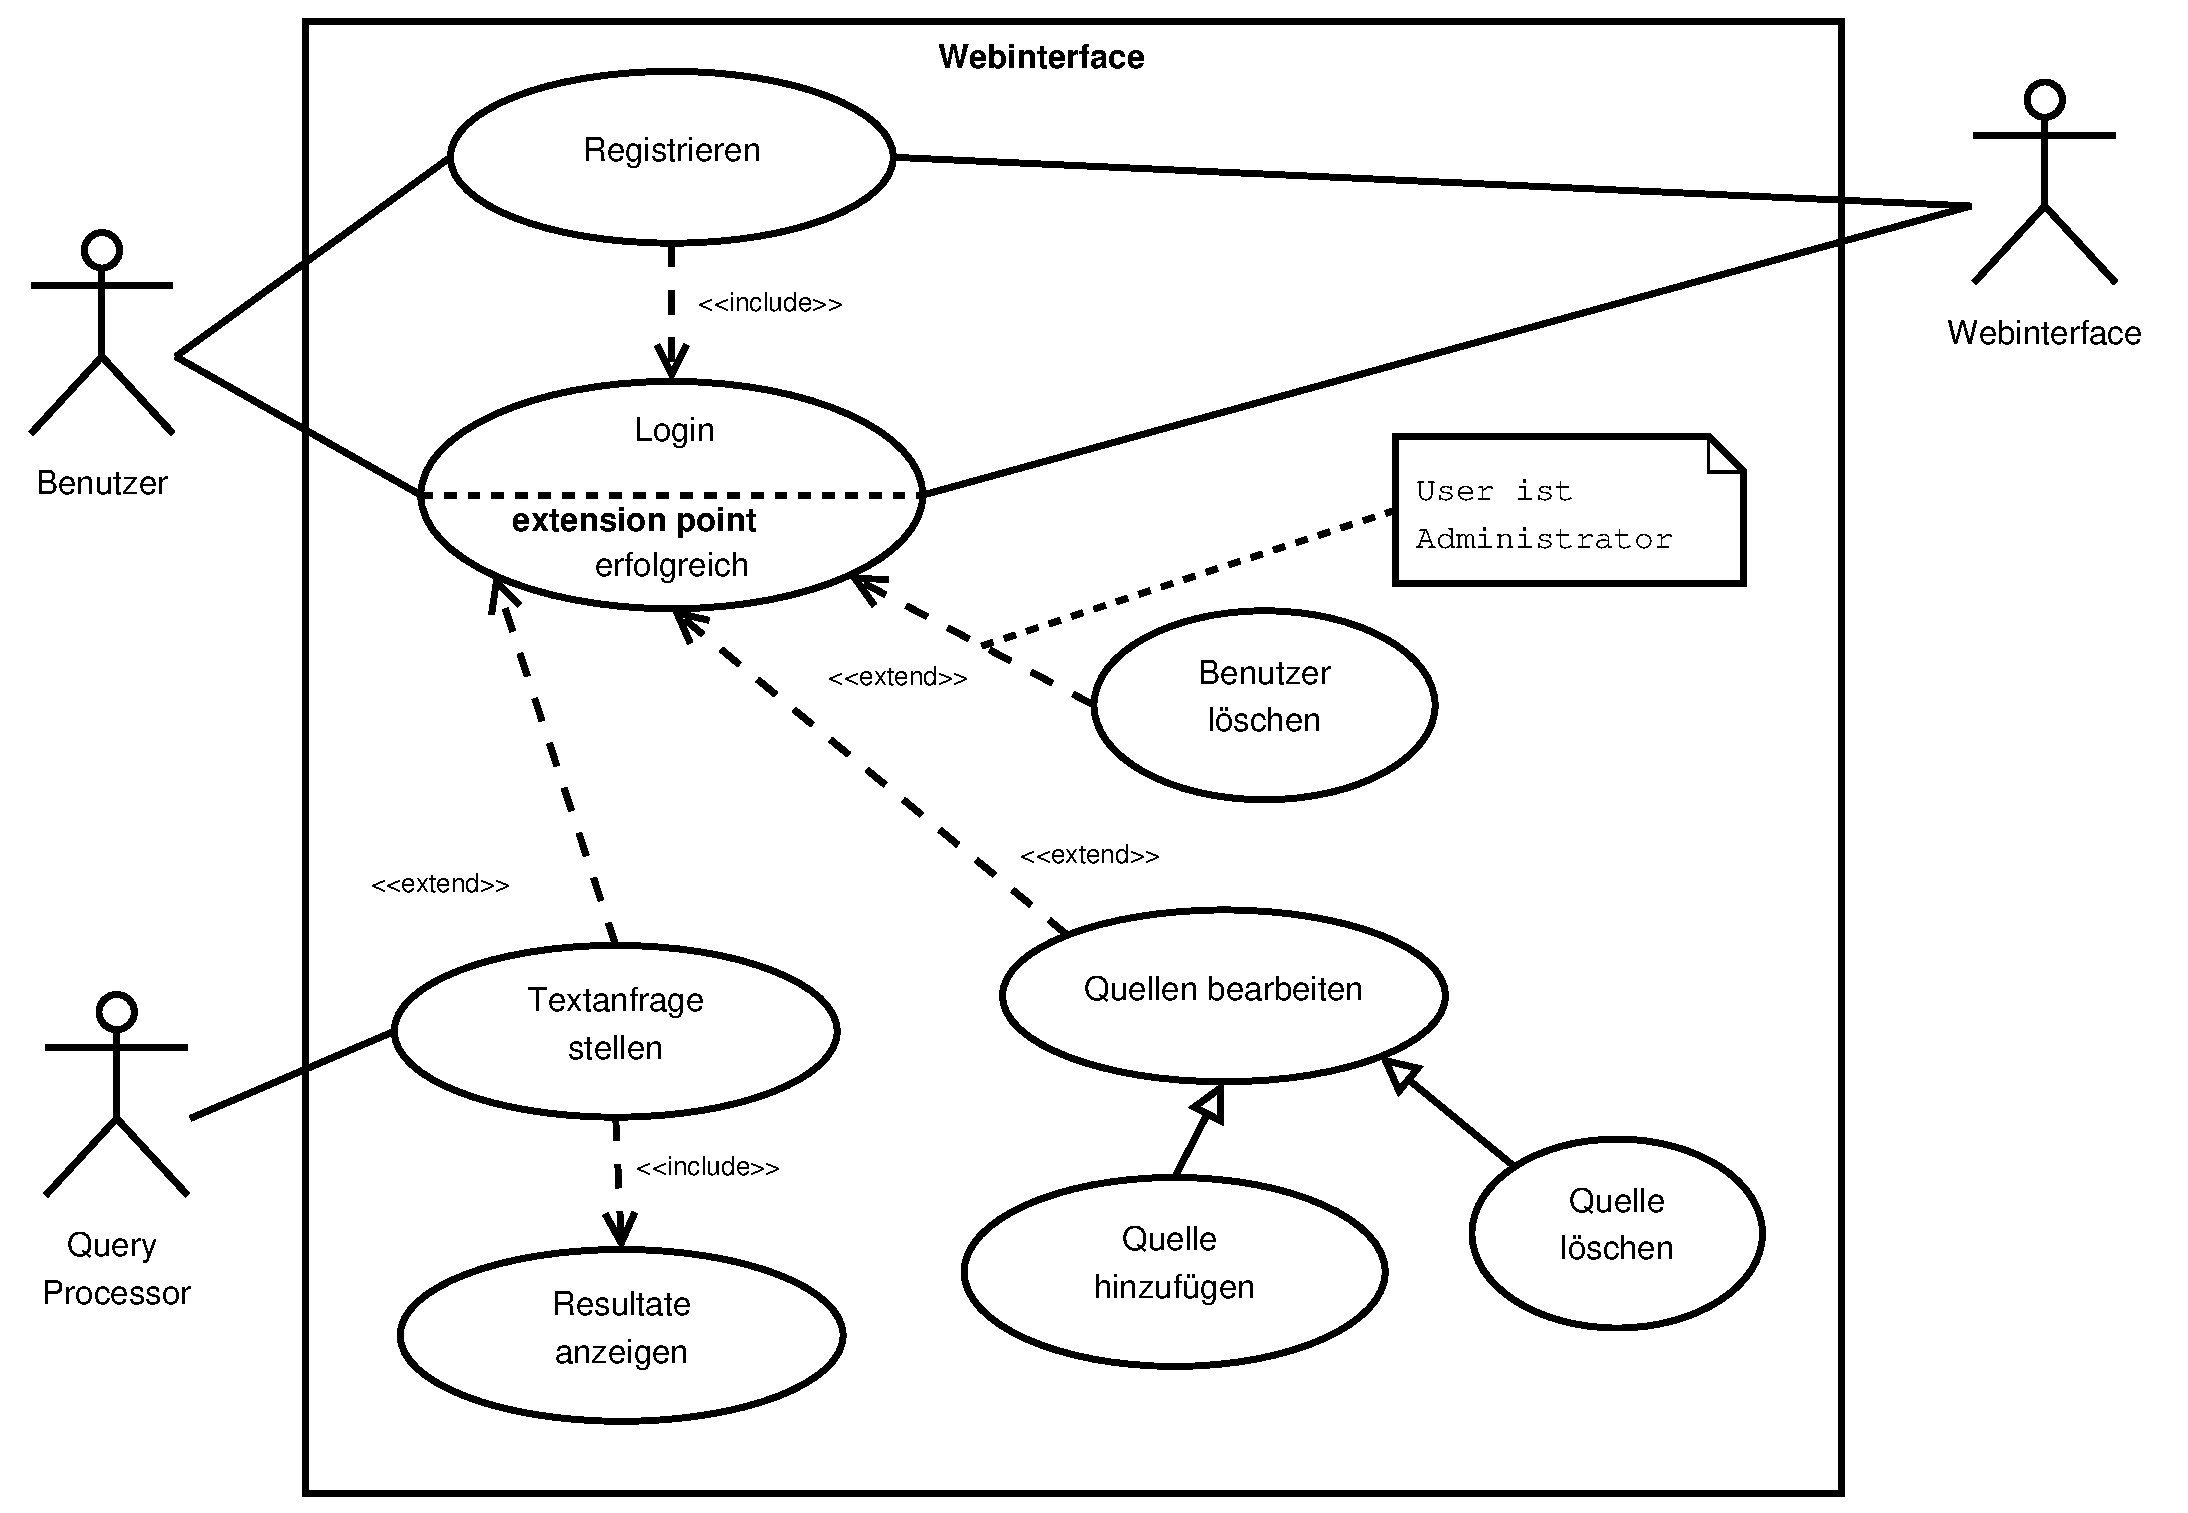
\includegraphics[width=1\textwidth]{Pflichtenheft/03_produktuebersicht/webinterface}
\caption{Use-Case, \textit{Webinterface} \label{uc-webinterface}}
\end{figure}

\FloatBarrier

Das Webinterface bietet weiterhin die Möglichkeit, direkt Textanfragen an der
Server zu stellen ohne einen Client mit Sprachschnittstelle zu nutzen.
Die Ergebnisse werden übersichtlich in Textform präsentiert, außerdem können
Debug-Informationen abgerufen werden.

